\section{Discussion}
\label{sec:discussion}

\subsection{Analysis}

Here, we provide an analysis on the upper bound on the number of instructions that can be executed, given the eBPF processor clock and the interface speed.

From Ethernet standard (IEEE 802.3)~\cite{EthernetStandard}, the preamble has 7 bytes and the start of frame delimiter (SFD) has 1 byte. The interframe gap (IFG) is composed of 12 bytes.
So, for every frame of X bytes, the link transmits (X+20) bytes, or (X+20)*8 bits. Thus, the number of frames per second (\#fps) to be processed is equal the interface speed (bps) divided by (frame\_size(bytes)+20)*8.

The time to process one frame is 1/\#fps.
For a single stage processor (clocks per instruction (CPI) equals 1), the processor can execute clock (Hz) instructions.
Suppose that the time to process a frame is spent only on the eBPF processor, the number of instructions that can be executed by a given interface speed and frame size is: clock(Hz)/\#fps.

\begin{figure}[htb]
\centering
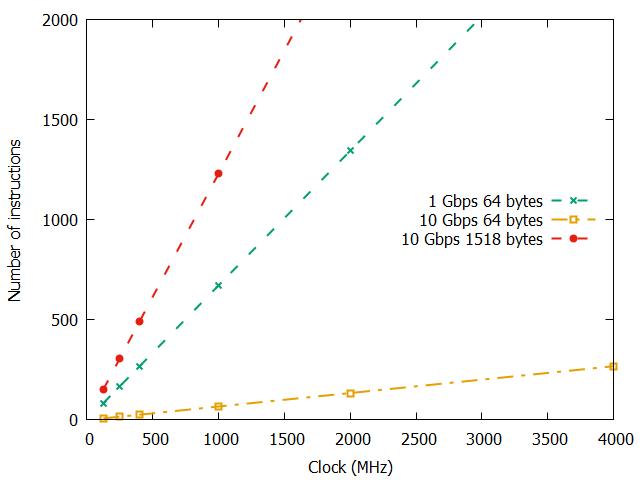
\includegraphics[width=1.\linewidth]{figures/numberInstructionsPerClock.png}
\caption{Maximum number of instructions that can be processed given CPU clock (MHz),  interface speed (Gbps), and frame size (bytes).}
\label{fig:instructionsPerClock}
\end{figure}

Figure~\ref{fig:instructionsPerClock} shows the upper bound of eBPF instructions that can be processed, given the eBPF processor clock in MHz, the interface speed in Gbps, and the frame size (bytes). The smaller is the frame size, the large is the number of frames to process. Thus, smaller frames require to be processed with fewer eBPF instructions. For 10 Gbps links, a frame size of 64 bytes, and 1 GHz clock, the maximum number of instructions is 67.
Current CPU desktops operate at near 4 GHz, which results in an upper bound of 268 instructions.


\subsection{Limitations}

% Nao sei se coloca esse paragrafo.
%
% Currently implementation only support one table for each matching type (LPM, exact-matching, array). In practice, this is not harmful since usually only one LPM table is required (for IP matching). Moreover, exact-matching table can incorporate many tables, as long as items do not share the same key. But, ideally, eBPFlow should receive an ELF file containing the structure of the tables and map them to hardware or a compiler would map logical lookup tables to physical tables~\cite{Lavanya2015CompilingTable}.

For a matching field that belongs to the OpenFlow standard, it might require only 1 flow rule and 1 TCAM lookup, while eBPFlow requires at least four instructions (one load of packet field, one load of the data value to be compared, one comparison and branch, one return value). But on the other hand, eBPFlow allows for logical expressions (not, and, or) and range comparison($>$,$<$). OpenFlow would require more rules and the number of rules (memory) is important in TCAM. Moreover, as shown in Figure~\ref{fig:instructionsPerClock}, spending some eBPF instructions, for example 4, to parse a packet is acceptable.

In current implement, the eBPF processor is a shared resource for all input queues.
We plan, for future work, to place an eBPF processor for each input queue. 
In this case, a NetFPGA with a larger number of cells is required.
Our system has already been designed to integrate multiple eBPF processors. This is the reason that, in our design, the instruction memory is already in another module separated from the eBPF processor. 
Instruction memory could be read in parallel by several eBPF processors simultaneously.

Currently eBPFLow implementation on NetFPGA SUME provides \marcos{XXXXX} throughput (Figure~\ref{fig:07result}). 
%This is due to the limitations of NetFPGA 1G platform. 
FPGAs are useful for prototyping and validating the hardware logic design~\cite{cofer2005rapid,sukhwani2017contutto}. 
The logic design for FPGA shares the same initial flow and methodology as ASIC design~\cite{kuon07measuring,ASICDesignFlow2005}. 
We leave eBPFlow over ASIC as future work.

